\documentclass{standalone}
\usepackage{tikz}
\usepackage{amsmath}

\begin{document}
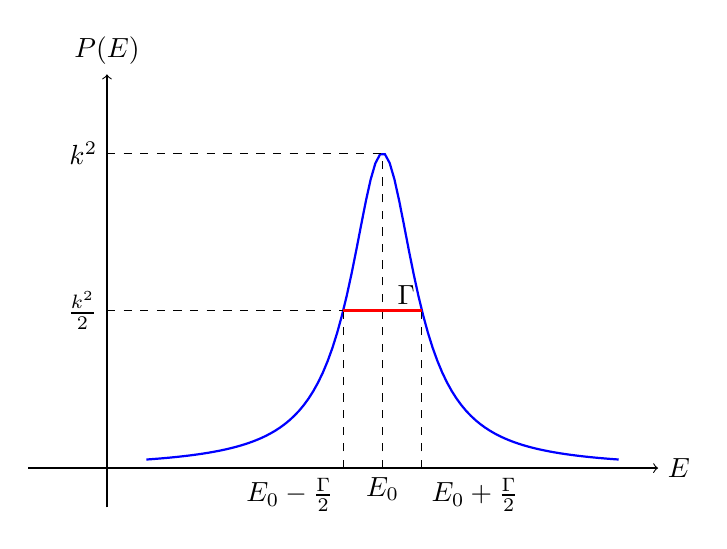
\begin{tikzpicture}
    % Ejes
    \draw[->] (-1,0) -- (7,0) node[right] {$E$};
    \draw[->] (0,-0.5) -- (0,5) node[above] {$P(E)$};

    % Curva (una campana simple)
    \draw[blue, thick, domain=0.5:6.5, samples=100] plot (\x, {(1/((\x-3.5)^2+(0.5)^2)});

    % Líneas verticales
    \draw[dashed] (3,0) node[below left] {$E_0 - \frac{\Gamma}{2}$} -- (3,2) ;
    \draw[dashed] (4,0)node[below right] {$E_0 + \frac{\Gamma}{2}$} -- (4,2) ;
    \draw[dashed] (3.5,0)node[below] {$E_0$} -- (3.5,4) ;

    % Línea horizontal en k^2/2
    \draw[dashed] (0,2) -- (3.5,2);
    \node[left] at (0,2) {$\frac{k^2}{2}$};

    % Línea roja horizontal para ancho de la curva
    \draw[red, thick] (3,2) -- (4,2);
    \node at (3.8,2.2) {$\Gamma$};

    % Líneas horizontales adicionales en la parte superior
    \draw[dashed] (0,4) -- (3.5,4);
    \node[left] at (0,4) {$k^2$};
\end{tikzpicture}
\end{document}
